\section{Processing raw images from
station}\hypertarget{raw-data-from-station}{}\label{raw-data-from-station} We think that the samples we are looking at in the current run (the fourth) on
ISS with ACE-M2 are undergoing phase separation and gelation, based on ground
studies and preliminary images from orbit. To understand how these samples
evolve over time, we perform nominally the same procedure---collecting images
from the same positions, magnifications, depths, at similar settings---each day
we run the experiment. In principle, then the images from successive days should
have the same (or at least very close) brightness and contrast, and should
overlay on top of each other exactly. To see whether this is happening in
practice, here is the raw sequence of 10x composite images of sample 22 (platter
2105, strip B618, well 4) taken on days 2, 3, 5, 8, 11 and 15:
\begin{figure}[h]
\begin{center}
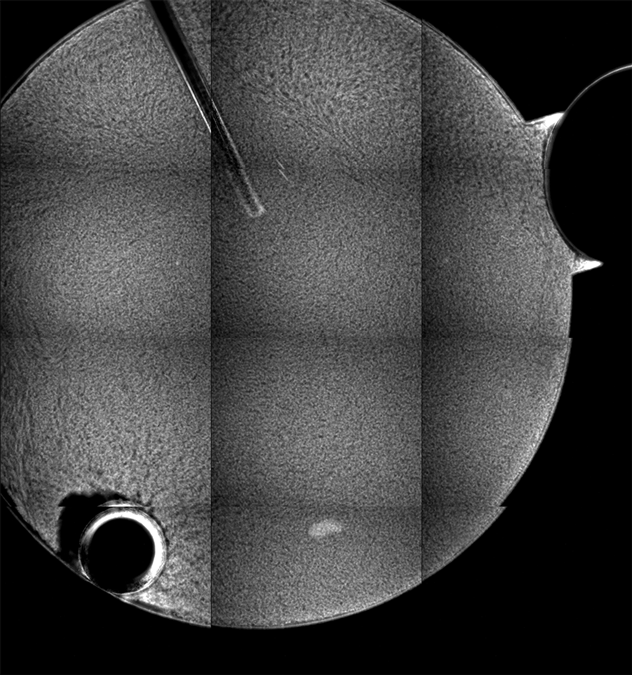
\includegraphics[width=\columnwidth]{./images/2014_07_27_ace_m2_run4_s22_gel/w9s22_10x_days02to15_resize.png}
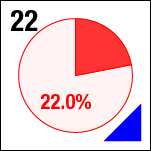
\includegraphics{./images/ace_m2_sample_tiles/sample22.png}
\caption{10x composite, raw images}
\end{center}
\end{figure}

The position shifts slightly, and the brightness changes. Clearly, the images
are not exactly aligned, and the motion distracts from being able to watch any
evolution in the sample, as well as interfering with any automated analysis.

\subsection{Pre-processing image
data}\hypertarget{pre-processing-image-data}{}\label{pre-processing-image-data} To fix these issues, I will align the images within the time sequence, and match
their brightnesses so that the intensity doesn't change so dramatically.

\subsubsection{Aligning the
images}\hypertarget{aligning-the-images}{}\label{aligning-the-images} The first major task is to align the images from subsequent days of data
collection. I first rename
the files, then in Photoshop CS6 import the set of images into separate layers
in a composite image, with {\tt File \textgreater{} Scripts \textgreater{} Load
Files into Stack...}, enabling the option to {\tt Attempt to Automatically Align
Source Images}. This works pretty well for these images, where the overall shape
of the well can guide the alignment algorithm.

This process is not fast, taking several seconds per image, but for just a
handful of images, it works well enough. By contrast, for BCAT, where we have
hundreds of frames, I create an image sequence movie in Adobe After Effects, and
use the tracking features there to far more quickly do the alignment.

I then crop the images so that there are no blank borders, and save the file as
a mult-layer {\tt .psd} file.

\subsubsection{Matching
intensities}\hypertarget{matching-intensities}{}\label{matching-intensities} For color images, the Photoshop feature {\tt Match Color...} is very good and
extremely helpful. In our case, however, grayscale images do not have the same
feature, and the option is unavailable. Instead, using a combination of {\tt
Levels} and ```Curves, I adjust each image to have the same mean (a little over
100 in 8-bit grayscale values) and standard deviation (about 60 8-bit grayscale
levels).

\subsubsection{Building the
animation}\hypertarget{building-the-animation}{}\label{building-the-animation} In the {\tt Timeline} palette, I {\tt Create Frame Animation}, then in the
drop-down menu select {\tt Make Frames from Layers}. The great thing about this
feature is that it otherwise doesn't affect anything about the image or its
layers. The final step is to export to an animated {\tt .gif} file, using the
{\tt Save for Web...} dialog box. There I reduce to final web resolution, and
create the final file:
\begin{figure}[h]
\begin{center}
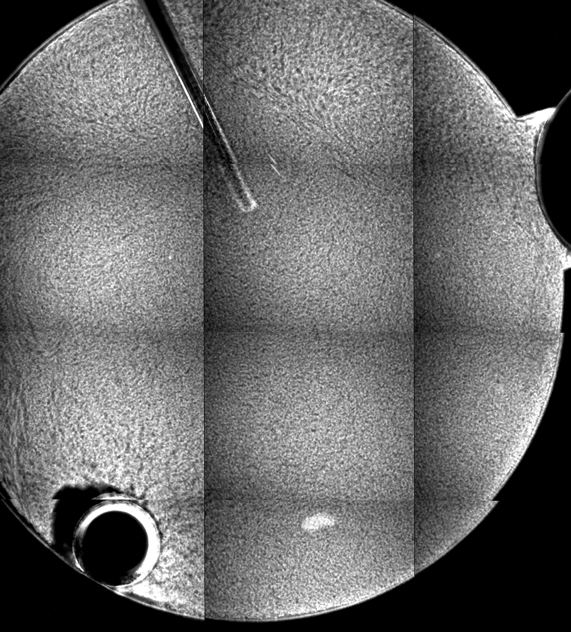
\includegraphics[width=\columnwidth]{./images/2014_07_27_ace_m2_run4_s22_gel/w9s22_10x_days02to15.png}
\end{center}
\caption{10x composite, aligned images}
\end{figure}

\clearpage

\subsection{Higher
magnification}\hypertarget{higher-magnification}{}\label{higher-magnification} I apply the same procedure to the higher-magnification 40x composite. First, the
raw data (just resized):
\begin{figure}[h]
\begin{center}
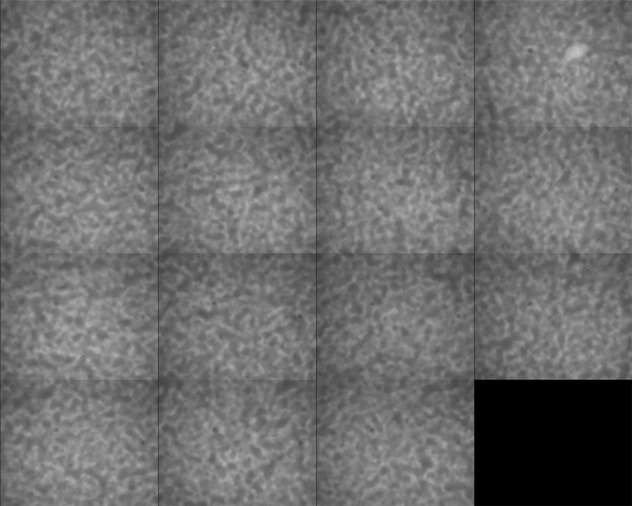
\includegraphics[width=\columnwidth]{./images/2014_07_27_ace_m2_run4_s22_gel/w9s22_40x_60um_days04to15_resize.png}
\end{center}
\caption{40x composite, raw images}
\end{figure}

And then the corrected version, where the aligned images have a mean of 128 and standard deviation of 40 8-bit grayscale levels:
\begin{figure}[h]
\begin{center}
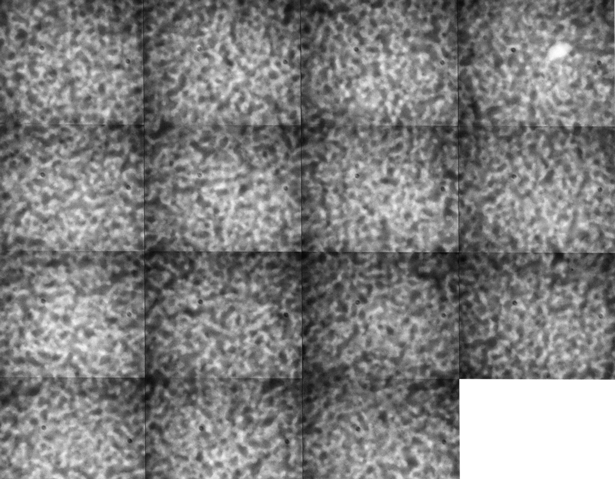
\includegraphics[width=\columnwidth]{./images/2014_07_27_ace_m2_run4_s22_gel/w9s22_40x_60um_days04to15.png}
\end{center}
\caption{40x composite, aligned images}
\end{figure}

%\subsection{Stage reproducibility or drift?}
Several things are apparent from these sequences. First, the stage is not
perfectly reproducible from a mechanical standpoint. The composites seem to move
around a little bit, likely due to mechanical backlash in the stage. Second,
intensities are not constant from day to day.